\begin{figure}[h]
\centering
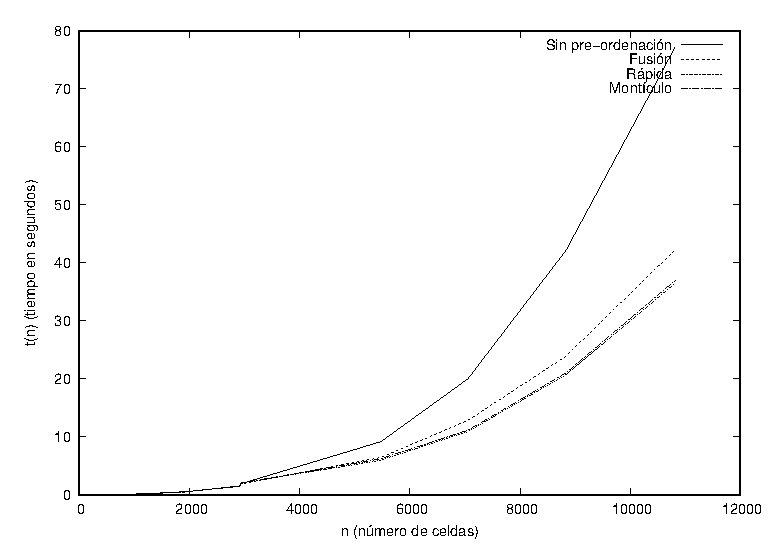
\includegraphics[width=0.5\linewidth]{./graphic}
\caption{Tiempos de ejecución para cada estrategia}
\label{fig:defenseValueCellsHead}
\end{figure}

Vemos como la peor es claramente la que no tiene pre-ordenación, y después la de fusión. Después, aunque muy similares, el montículo parece ser algo mejor que la ordenación rápida. Para la medición de tiempos se ha usado el siguiente código:

\begin{lstlisting}
void DEF_LIB_EXPORTED placeDefenses3(bool** freeCells, int nCellsWidth, int nCellsHeight, float mapWidth, float mapHeight
              , List<Object*> obstacles, List<Defense*> defenses) {

    float cellWidth = mapWidth / nCellsWidth;
    float cellHeight = mapHeight / nCellsHeight; 

	cronometro c;
    long int r = 0;
    double e_abs = 0.01, e_rel = 0.001;

    c.activar();
    do {
		algoritmoVorazSinOrdenar(nCellsWidth, nCellsHeight, freeCells, mapWidth, mapHeight, obstacles, defenses);
		
		++r;
    } while(c.tiempo() < e_abs/e_rel + e_abs);
    c.parar();
    double t1 = c.tiempo() / r;

    r = 0;
    c.activar();
    do {
	    algoritmoVorazFusion(nCellsWidth, nCellsHeight, freeCells, mapWidth, mapHeight, obstacles, defenses);
		
		++r;
    } while(c.tiempo() < e_abs/e_rel + e_abs);
    c.parar();

    double t2 = c.tiempo() / r;

    r = 0;
    c.activar();
    do {
		algoritmoVorazRapida(nCellsWidth, nCellsHeight, freeCells, mapWidth, mapHeight, obstacles, defenses);
		
		++r;
    } while(c.tiempo() < e_abs/e_rel + e_abs);
    c.parar();

    double t3 = c.tiempo() / r;

    r = 0;
    c.activar();
    do {
		algoritmoVorazMont(nCellsWidth, nCellsHeight, freeCells, mapWidth, mapHeight, obstacles, defenses);

		++r;
    } while(c.tiempo() < e_abs/e_rel + e_abs);
    c.parar();

    double t4 = c.tiempo() / r;

    std::cout << (nCellsWidth * nCellsHeight) << '\t' << t1 << '\t' << t2 << '\t' << t3 << '\t' << t4 << std::endl;
}
\end{lstlisting}

Esta salida es la que necesita el comando \emph{make data}, que es el que he usado, y a continuación \emph{make plot} para generar la gráfica. Posteriormente se convirtión a pdf para poder integrarla en la memoria.
